\documentclass[
	%parspace, % Add vertical space between paragraphs
	%noindent, % No indentation of first lines in each paragraph
	%nohyp, % No hyphenation of words
	%twoside, % Double sided format
	%draft, % Quicker draft compilation without rendering images
	%final, % Set final to hide todos
]{elteikthesis}[2024/04/26]

\setcounter{secnumdepth}{3}
\setcounter{tocdepth}{3}

\usepackage{tabularx}
\usepackage{booktabs}
\renewcommand{\arraystretch}{1.25}
\usepackage{tikz}
\usetikzlibrary{shapes,arrows,positioning}

\tikzset{
  wf/.style={font=\sffamily\footnotesize},
  wf frame/.style={draw=black!70, line width=0.8pt, fill=white},
  wf bar/.style={draw=black!40, fill=black!8},
  wf box/.style={draw=black!50, fill=black!3, rounded corners=2pt},
  wf btn/.style={draw=black!60, fill=black!12, rounded corners=3pt, inner sep=3pt},
  wf input/.style={draw=black!60, fill=white, minimum height=0.55cm, inner sep=3pt, anchor=west},
  wf line/.style={black!25, line width=3pt, line cap=round},
  wf state/.style={draw=black!70, circle, minimum size=0.75cm, inner sep=0pt},
  wf mark/.style={circle, fill=black!80, text=white, font=\sffamily\scriptsize\bfseries,
                  inner sep=1pt, minimum size=0.42cm},
}

\lstset{
    float=false,
    numbers=none,
    literate={á}{{\'a}}1 {é}{{\'e}}1 {í}{{\'i}}1 {ó}{{\'o}}1 {ö}{{\"o}}1
             {ő}{{\H{o}}}1 {ú}{{\'u}}1 {ü}{{\"u}}1 {ű}{{\H{u}}}1
             {Á}{{\'A}}1 {É}{{\'E}}1 {Ö}{{\"O}}1 {Ü}{{\"U}}1
}

\newcommand{\kep}[2][]{%
  \IfFileExists{images/#2}%
    {\includegraphics[#1]{#2}}%
    {\fbox{\parbox[c][4cm][c]{0.8\textwidth}{\centering Hiányzó kép: \texttt{\detokenize{#2}}}}}%
}

\title{Interaktív webalkalmazás a Számításelmélet alapjai I--II tárgyhoz}
\date{2026}

\author{Szabó Anna}
\degree{programtervező informatikus BSc}

\supervisor{Tichler Krisztián}
\affiliation{egyetemi adjunktus}

\university{Eötvös Loránd Tudományegyetem}
\faculty{Informatikai Kar}
\department{Algoritmusok és Alkalmazásaik Tanszék}
\city{Budapest}
\logo{elte_cimer_szines}

\addbibresource{szakdolgozat.bib}

\begin{document}

\documentlang{hungarian}

%\listoftodos[\todolabel]

\maketitle

\includepdf{temabejelento.pdf}
%\includepdf{mi_nyilatkozat.pdf}

\tableofcontents
\cleardoublepage

\chapter{Bevezetés}
\label{ch:intro}

\section{Motiváció és problémafelvetés}

Az egyetemi évek alatt számos olyan tárgyat tanulunk, amelyek megértése
jelentős absztrakciós képességet igényel, és sokszor nagyon elvontnak,
nehezen megfoghatónak tűnnek. Hallgatóként én is többször találkoztam olyan
tananyaggal, ahol a fogalmak és folyamatok elsőre nehezen voltak értelmezhetők.
Különösen igaz ez azokra a témákra, amelyekben egy rendszer működésének megértéséhez
több egymásra épülő állapotot vagy lépést kell végigkövetni.
Az ilyen absztrakt gondolatmenetek papíron gyakran nehezen követhetők,
hiszen egy folyamat vagy modell működését látni egészen más élmény,
mint pusztán olvasni róla.

Erre jó példa a Számításelmélet alapjai I--II. tárgy,
amely olyan témaköröket dolgoz fel, mint a formális nyelvek,
a grammatikák, a véges automaták, a reguláris kifejezések,
a veremautomaták vagy a Turing-gépek.
Ezek a fogalmak a hallgatók számára gyakran nehezen értelmezhetők, mivel
működésük és viselkedésük hagyományos tananyagok segítségével nem mindig
szemléltethető egyszerűen.
A tananyag elsajátításához általában előadásanyagok, prezentációk és
órai jegyzetek állnak rendelkezésünkre. Bár ezek fontos szerepet
töltenek be az oktatásban, és ezek adják a tudásunk alapját, a
mélyebb megértés sokszor a gyakorlatokra, illetve az önálló otthoni
tanulásra hárul.

Saját tapasztalatom szerint ezeknél a témáknál a megértés kulcsa
éppen az, hogy az ember minden állapotot és lépést végigkövet. Papíron
ez azonban lassú: gyakran minden állapotot külön le kell rajzolni, egy
elrontott lépés után pedig elölről kell kezdeni. Ezért az ilyen
témáknál mi, hallgatók gyakran nagyon sok időt töltünk az anyag önálló
feldolgozásával.

A szakdolgozat erre a problémára kíván megoldást nyújtani egy olyan
webalapú oktatási rendszer fejlesztésével, amely a tantárgy
legfontosabb témaköreit interaktív, vizualizációra épülő formában
dolgozza fel. A rendszer a témakörökhöz elméleti összefoglalót,
lépésenként követhető szimulációkat (például determinisztikus véges
automata, grammatikai levezetés) és önellenőrző feladatokat kínál,
így a lépésenkénti követés gyorssá és hibatűrővé válik.
% TODO: a felsorolt példákat a végén egyeztetni az elkészült modulokkal

\section{Célkitűzések}
A szakdolgozat célja egy interaktív és vizualizációs oktatási webalkalmazás
tervezése és fejlesztése, amely támogatja a hallgatókat a Számításelmélet
alapjai I--II. tantárgy témaköreinek elsajátításában.
A fejlesztés során olyan rendszer létrehozása a cél,
amely egyetlen felületen egyesíti az elméleti háttéranyagot, a vizuális
szemléltetést és az interaktív gyakorlási lehetőségeket. A hallgatók így
nem csupán olvashatnak az egyes modellekről és algoritmusokról, hanem
működésüket lépésről lépésre követhetik, és saját bemenetek segítségével
ki is próbálhatják.
A rendszer fontos célja továbbá, hogy támogassa az önálló tanulást,
valamint segítséget nyújtson a gyakorlásban és a vizsgákra való
felkészülés során.
A kitűzött célok az alábbiakban foglalhatók össze:

\begin{itemize}
    \item a Számításelmélet alapjai I--II. főbb témaköreinek feldolgozása;
    \item elméleti összefoglaló a tárgy jelöléseivel, matematikai képletekkel;
    \item saját felhasználói bemenetre működő, lépésenként követhető szimulációk;
    \item azonnali visszajelzés és önellenőrzés: kvízek, feladatok;
    \item böngészőből, telepítés nélkül elérhető felület;
    \item bővíthető, moduláris alkalmazásarchitektúra kialakítása.
\end{itemize}

\section{Hatókör és korlátok}

\subsection{Hatókör}

% TODO: a számokat és a modullistát a végén egyeztetni a kóddal
% (packages/content/src/topics, apps/web/src/modules/index.tsx)
A szakdolgozat egy webalapú, egyfelhasználós oktatási alkalmazás
tervezését és megvalósítását foglalja magában, amely a Számításelmélet
alapjai I--II. tárgy témakörét dolgozza fel Minden témakörhöz elméleti összefoglaló
tartozik, amelyet több helyen interaktív modul egészít ki.

rendszer összesen x témakört dolgoz fel, amelyek xx nagyobb csoportba sorolhatók: 
alapfogalmak, reguláris nyelvek, környezetfüggetlen nyelvek és környezetfüggő nyelvek...
 Az egyes témakörökhöz elméleti összefoglalók, valamint interaktív modulok tartoznak, 
 amelyek lehetővé teszik a modellek és algoritmusok működésének lépésről lépésre történő megfigyelését.
 
A megvalósított modulok közé tartozik többek között a DVA-szimulátor, a grammatikalevezető, a Chomsky-osztályozó, a 3-as normálforma vizualizáló, a reguláris kifejezés ellenőrző, a nyelvfelfedező, a szójáték és a kvízrendszer.

% TODO: NDVA-szimulátor elkészült? Ha igen, kerüljön a fenti listába
% TODO: ha a témakör-táblázat bekerül a fejlesztői dokumentációba, ide hivatkozás:
% A témakörök és modulok részletes áttekintését a \ref{tab:temakorok}.~táblázat tartalmazza.

A dolgozat része a fejlesztői dokumentáció, vagyis
a rendszer architektúrájának bemutatása, a tervezés
dokumentálása, az implementáció ismertetése, valamint a megvalósított
funkciók tesztelése és értékelése. Végül egy felhasználói dokumentáció
is készül, amely a rendszer használatát segíti.

\subsection{Korlátok}

A dolgozat keretében megvalósított rendszer oktatási célú
prototípusnak tekinthető. Bár alkalmas a tanulás támogatására, nem
célja egy teljes körű e-learning vagy tanulmányi rendszer kiváltása.
A rendelkezésre álló idő és fejlesztési kapacitás miatt a tantárgy teljes
 tananyagának részletes feldolgozása nem valósul meg. 
 A rendszer elsősorban azokra a témakörökre összpontosít, amelyek különösen jól támogathatók vizualizációval
  és interaktív szimulációkkal.
A Számításelmélet alapjai II. tárgy csak részben kerül feldolgozásra.
A szimulációk kisméretű, véges bemenetekre lettek tervezve.
Nincs felhasználókezelés, a haladás nem tárolódik központilag.

\subsection{Feltételezések}

A rendszer használata modern webböngésző meglétét feltételezi. A
felhasználók rendelkeznek alapvető informatikai ismeretekkel, valamint
a Számításelmélet alapjai I--II. tárgy követéséhez szükséges
előismeretekkel. Mivel a tananyag az előadásokra épül, azokat nem
helyettesíti, hanem kiegészíti. A tervezés során feltételezem, hogy a webes
technológiák és a kliensoldali vizualizációs megoldások elegendő
teljesítményt biztosítanak az interaktív modulok futtatásához.

\section{A dolgozat fő eredményei}

\begin{itemize}
    \item egy interaktív, webalapú oktatási rendszer tervezése és
          megvalósítása a Számításelmélet alapjai I--II. tárgy támogatására;
    \item olyan interaktív vizualizációs és szimulációs eszközök fejlesztése, amelyek
     lehetővé teszik a hallgatók számára a számításelméleti modellek működésének lépésről 
     lépésre történő követését;
    \item a tananyag egységes, típusos, blokkalapú tartalommodellbe
          szervezése;
    \item moduláris és bővíthető szoftverarchitektúra kialakítása;
    \item interaktív szimulációs és kiértékelő mechanizmusok fejlesztése;
    \item a rendszer tervezésének, implementációjának és tesztelésének
          dokumentálása.
\end{itemize}

A dolgozat eredménye egy olyan oktatási segédeszköz, amely a
hagyományos tananyagokat kiegészítve támogatja az önálló tanulást, a
szemléletesebb megértést és a gyakorlati tapasztalatszerzést.

\section{A dolgozat felépítése}
A dolgozat két fő részre tagolódik.
A felhasználói dokumentáció a rendszer felépítését és használatát
ismerteti a végfelhasználó szemszögéből. Ez kiterjed az egyes modulok
bemutatására és az interaktív, szimulációs eszközök használatára
példákon keresztül.

A fejlesztői dokumentáció a műszaki hátteret mutatja be. Itt kap helyet
a követelményelemzés, a tervezési döntések indoklása, az architektúra
ismertetése és az implementáció bemutatása. Ezenkívül ez a rész tér ki
a tesztelési folyamatokra, valamint a jövőbeni fejlesztési irányokra
és bővítési lehetőségekre is.
A dolgozatot egy rövid értékelés zárja.

\cleardoublepage

\chapter{Felhasználói dokumentáció}
\label{ch:user}

\section{A program célja} 
Ez a fejezet a rendszer használatát mutatja be a felhasználó szemszögéből. Ismerteti az alkalmazás elérésének és telepítésének módját, bemutatja a főbb funkciókat, valamint segítséget nyújt azok használatához. A fejezet végén az ismert korlátozások, az elérhetőségi információk és a hibaelhárítással kapcsolatos tudnivalók találhatók.
\mbox{}

\section{Rendszerkövetelmények és indítás}
\subsection{Rendszerkövetelmények}
A rendszer online eléréséhez nincs különösebb hardverigény.
Támogatott böngészők: Google Chrome, Microsoft Edge és Mozilla Firefox.
Az online változat használatához internetkapcsolat és egy támogatott böngésző szükséges. A helyi futtatáshoz ezen felül a 2.2.3 fejezetben ismertetett szoftverek telepítése is szükséges.

\mbox{}

\subsection{Az alkalmazás elérése}
Az alkalmazás GitHub Pages-en van közzétéve, és az alábbi linken érhető el:
\begin{center}
  \url{https://szaboanna21.github.io/thesis/#/}
\end{center}

\mbox{}

\subsection{Helyi futtatás}
A felület internetkapcsolat nélkül, lokálisan is futtatható a felhasználó számítógépén.
A futtatáshoz az alábbi szoftverek szükségesek:
\begin{itemize}
  \item \textbf{Node.js 24} (\url{https://nodejs.org}), amely lehetővé teszi a JavaScript alapú alkalmazások futtatását a számítógépen. 
  \item \textbf{pnpm 12.6}: \texttt{npm install -g pnpm@12.6.0}, amely automatikusan telepíti és kezeli az alkalmazás működéséhez szükséges csomagokat.

Hogyha, ezek már telepítve vannak, az alkalmazás az alábbi lépésekkel indítható el:

\begin{enumerate}
  \item A projekt forráskódjának letöltése: 
  \begin{lstlisting} 
    git clone https://github.com/SZaboAnna21/thesis.git
  \end{lstlisting} 

  \item Belépés a projekt könyvtárába: 
  \begin{lstlisting} 
    cd thesis/Fotoc-helper
  \end{lstlisting} 
  \item Az alkalmazás működéséhez szükséges csomagok telepítése:
  \begin{lstlisting} 
    pnpm install
  \end{lstlisting} 
  Ez a lépés automatikusan letölti a program futtatásához szükséges kiegészítő könyvtárakat.
  \item Indítás: 
  \begin{lstlisting} 
    ppnpm --filter web dev
  \end{lstlisting}  
  \item A sikeres indítást követően az alkalmazás a böngészőből a \texttt{http://localhost:5173} címen érhető el.
\end{enumerate}

\mbox{}
A helyi futtatás elsősorban fejlesztői vagy tesztelési célokat szolgál. 
Azoknak a felhasználóknak, akik kizárólag használni szeretnék az alkalmazást, 
elegendő az online változat megnyitása a 2.2.2 fejezetben szereplő címen.

\section{A felület áttekintése}

\subsection{Főoldal és navigáció}
A fenti „Az alkalmazás elérése” szekcióban bemutatott hivatkozás a rendszer főoldalára navigálja a felhasználót.
 A főoldal rövid ismertetőt tartalmaz az alkalmazás céljáról és használatáról, valamint innen indulva érhető el az összes témakör.
A navigációt a lap tetején elhelyezett, minden oldalon elérhető fejléc biztosítja. 
A fejléc bal oldalán található a házikó ikon, amely a főoldalra vezet vissza.
 Mellette kettő lenyíló menü érhető el: 
 \begin{itemize}

    \item Számításelmélet I
    \item Számításelmélet II.

 \end{itemize}


A Számításelmélet I menü az első féléves anyagot, míg a Számításelmélet II menü a második félév témaköreit tartalmazza.
 A témakörök menün belüli sorrendje az előadások haladását követik,
 így a hallgatók a tananyag felépítésének megfelelően ezt szépen követve, járhatják be az egyes fejezeteket.

 A lenyíló listában pici pipa jelöli azokat az oldalakat,
  amelyeket a felhasználó már megnyitott.
 A menü alján egy számláló mutatja a haladást, „Megnyitva: 3 / 16”, tájékoztatást adva arról, hogy az adott menüből, (számításelmélet I. vagy II. csoportból ) hány oldala került már megtekintésre/feldolgozásra.
\begin{figure}[H] \centering \fbox{ \includegraphics[width=0.5\textwidth]{images/userdoksi_haladas.png} } \caption{A témakörválasztó menü haladáskövető funkciója} \label{fig:menu_haladas} \end{figure}


\newpage
A két menü által lefedett témakörök összefoglalása az alábbi táblázatban látható:


\begin{table}[H]
\centering
\begin{tabular}{p{0.46\textwidth} p{0.46\textwidth}}
\toprule
\textbf{Számításelmélet I} & \textbf{Számításelmélet II} \\
\midrule
Alapok 1: ábécé, szavak, műveletek        & Nulladrendű és elsőrendű logika \\
Alapok 2: nyelvek és műveleteik           & Turing-gépek \\
Generatív grammatikák                     & Számosság és eldönthetetlenség \\
Chomsky-hierarchia                        & Bonyolultsági osztályok \\
Lineáris grammatikák és a 3-as normálforma & NP-teljesség \\
Reguláris kifejezések                     & \\
Determinisztikus véges automata           & \\
Nemdeterminisztikus véges automata        & \\
Minimális automata és Myhill--Nerode tétel & \\
Reguláris kifejezések és automaták        & \\
Kis Bar-Hillel lemma                      & \\
Redukált grammatika és Chomsky-normálforma & \\
CYK algoritmus                            & \\
Veremautomata                             & \\
Nagy Bar-Hillel lemma                     & \\
Környezetfüggő és 0-típusú nyelvek        & \\
\bottomrule
\end{tabular}
\caption{Az alkalmazásban elérhető témakörök}
\label{tab:temakorok}
\end{table}

A fejlécben lévő ház ikonra kattintva a user bármikor, bármely oldalról, visszatérhet a főoldalra, így a navigáció a rendszer minden pontján egyszerűen elérhető.

\begin{figure}[H]
    \centering
    \includegraphics[width=0.7\textwidth]{images/userdoksi_fooldal1.png}
    \caption{Főoldal és megnyitott témakörválasztó menü (A Számításelmélet I)}
    \label{fig:főoldal menü1}
\end{figure}
% Mit mutass be:
%   - ragadós fejléc: FOTOC logó/ikon (home link), két lenyíló menü (Számításelmélet I / II), sötét–világos mód kapcsoló
%   - a lenyíló lista: témakörök neve, pipajel (✓) a már megnyitottaknál, "Megnyitva: X / Y" számláló alul
%   - a főoldal hero szövege (rövid leírás, mi a FOTOC, hogyan induljunk el)
% Kérdések: Milyen témakörök érhetők el? Hogyan lehet navigálni közöttük? Mit lát a felhasználó első megnyitáskor?
% Képernyőkép: főoldal + nyitott lenyíló menü
\mbox{}

\subsection{Egy témakör oldala}
% Mit mutass be:
%   - morzsaútvonal fejléc (pl. "Számításelmélet I > Reguláris nyelvek > DFA")
%   - nagy cím, alatta elméleti összefoglaló (TheoryRenderer rendereli: szöveg, képletek, definíciók)
%   - "Próbáld ki!" szekció – az interaktív modul (nem minden témakörnek van)
%   - "Teszteld magad!" szekció – kvízkérdések (nem minden témakörnek van)
% Kérdések: Milyen típusú tartalmak jelennek meg az elméleti részben? Mi történik ha nincs modul / nincs kvíz?
% Képernyőkép: egy teljes témakör oldal (pl. DFA), jelölve a három részt

A témakörök oldalai nagyjából mind egységes felépítést követnek.
Az oldal tetején egy úgynevezett morzsaútvonal (breadcrumb) segíti a tájékozódást,
 amely megmutatja, hogy a felhasználó a tananyag mely részén jár.
 
A fejlécben található navigációs elemek a témakörök oldalain is elérhetők.
 Segítségükkel a felhasználó bármikor visszatérhet a főoldalra, vagy átválthat egy másik témakörre.
Az oldal fő részét az elméleti összefoglaló alkotja. 
Ez tartalmazza az adott témakör megértéséhez szükséges definíciókat, tételeket, példákat, valamint matematikai képleteket és jelöléseket.

Az elméleti tartalom célja, hogy röviden összefoglalja az előadások legfontosabb fogalmait, és alapot biztosítson az interaktív feladatok használatához.

Egyes témakörök esetén az elméleti rész alatt egy „Próbáld ki!” szekció is megjelenik.

Ez egy interaktív szimulációt vagy vizualizációt tartalmaz, amely lehetővé teszi a tananyag valamilyen gyakorlati kipróbálását.
Egyes szimulációk saját példák megadását is lehetővé teszik, így a felhasználó a tananyag működését tetszőleges bemeneteken is kipróbálhatja, módosíthatja a bemenetet, és lépésről lépésre követheti az algoritmusok/automaták működését.

Azoknál a témaköröknél, ahol ellenőrző kérdések állnak rendelkezésre, az oldal alján egy „Teszteld magad!” szekció található. A kvízkérdések segítségével a hallgató azonnali visszajelzést kaphat arról, hogy mennyire sajátította el az adott témakör anyagát.
A kvízek elsősorban a szimulációval nehezebben szemléltethető, elméletibb témaköröknél jelennek meg
. Minden témakör legalább egy kiegészítő elemet tartalmaz, amely vagy interaktív szimuláció, vagy kvíz formájában jelenik meg.


A \ref{tab:temakorok}. táblázat összefoglalja az egyes témakörökhöz tartozó interaktív modulokat és kvízeket.
\begin{table}[H]
\centering
\small
\begin{tabular}{p{0.52\textwidth} p{0.26\textwidth} c}
\toprule
\textbf{Témakör} & \textbf{Interaktív modul} & \textbf{Kvíz} \\
\midrule
\multicolumn{3}{l}{\textit{Számításelmélet I}} \\
\midrule
Alapok 1: ábécé, szavak, műveletek        & Szójáték              & ---         \\
Alapok 2: nyelvek és műveleteik           & ---                    & \checkmark  \\
Generatív grammatikák                     & Grammatika levezető    & ---         \\
Chomsky-hierarchia                        & Chomsky-osztályozó    & ---         \\
Lineáris grammatikák és a 3-as normálforma & 3-as normálforma      & ---         \\
Reguláris kifejezések                     & Regex ellenőrző       & ---         \\
Determinisztikus véges automata           & DVA szimulátor        & ---         \\
Nemdeterminisztikus véges automata        & NVDA labor            & ---         \\
Minimális automata és Myhill--Nerode tétel & Minimalizáló          & ---         \\
Reguláris kifejezések és automaták        & ---                   & \checkmark  \\
Kis Bar-Hillel lemma                      & ---                   & \checkmark  \\
Redukált grammatika és Chomsky-normálforma & CF levezetés          & \checkmark  \\
CYK algoritmus                            & CYK vizualizátor      & ---         \\
Veremautomata                             & Veremautomata labor   & ---         \\
Nagy Bar-Hillel lemma                     & ---                   & \checkmark  \\
Környezetfüggő és 0-típusú nyelvek        & ---                   & \checkmark  \\
\midrule
\multicolumn{3}{l}{\textit{Számításelmélet II}} \\
\midrule
Nulladrendű és elsőrendű logika           & Logika labor          & ---         \\
Turing-gépek                              & Turing-gép szimulátor & ---         \\
Számosság és eldönthetetlenség            & ---                   & \checkmark  \\
Bonyolultsági osztályok                   & ---                   & \checkmark  \\
NP-teljesség                              & ---                   & \checkmark  \\
\bottomrule
\end{tabular}
\caption{Az alkalmazásban elérhető témakörök interaktív moduljaikkal és kvízeikkel}
\label{tab:temakorok}
\end{table}

\mbox{}

\subsection{Haladáskövetés és megjelenés} 
Az alkalmazás automatikusan nyomon követi, 
hogy a felhasználó melyik témaköröket nyitotta már meg. 
Egy témakör első megnyitását követően a navigációs menüben egy pipa jelenik meg az adott oldal mellett a lenyíló mneüben.
 A menü alján található számláló megmutatja, hogy az adott témakörcsoportból hány oldal került már megnyitásra.
  Ez segítséget nyújt a tananyag feldolgozásának követésében. 
  A fejléc jobb oldalán található nap/hold ikon, ennek segítségével a felhasználó bármikor válthat a világos és a sötét megjelenési mód között.
 A választott beállításokat és haladást az alkalmazás megjegyzi, ezért a következő megnyitáskor is megmaradnak. 
  A haladási adatok és a megjelenési mód beállításai az adott böngészőben kerülnek tárolásra. 
  Emiatt másik böngésző vagy eszköz használata esetén vagy incognito módban ezek az adatok
  nem kerülnek automatikusan átvitelre. 
  A tárolt adatok a böngésző helyi adatainak törlésével visszaállíthatók alaphelyzetbe.
\mbox{}

\section{Interakív modulok használata}
Az alkalmazás több témakörhöz interaktív modult biztosít.
 Ezek a modulok, az adott témakörhöz kapcsolódó automaták, algoritmusok és egyéb számításelméleti 
 modellek kipróbálását biztosítja.
A következő alfejezetekben az egyes interaktív modulok használata olvasható,
 beleértve a megadható bemeneteket, a vezérlési lehetőségeket és az eredmények értelmezését.
 
\newpage 
\subsection{Szóműveletek}
% Mit mutass be: (LanguageExplorer + WordPlayground komponensek)
%   - LanguageExplorer: automata vagy grammatika által generált/elfogadott szavak böngészése,
%     szűrés hossz szerint, példaszavak listázása
%   - WordPlayground: szabad szó-tesztelés – adott automatán vagy grammatikán próbálhat szavakat
% Kérdések: Véges vagy végtelen szólistát mutat? Hogyan lehet szűrni? Mi a különbség a két almodul között?
Az első és talán a legegyszerűbb modul a legelső, vagyis az "Alapok 1: ábécé, szavak, műveletek" témát egészíti ki. 
A modul az alábbi szóműveletek eredményét jeleníti meg egy megadott szó alapján: \begin{itemize} \item hossz ($|u|$), \item tükörkép ($u^R$), \item konkatenáció egy másik szóval ($uv$), \item hatványozás ($u^n$), \item prefixek és valódi prefixek, \item szuffixek és valódi szuffixek. \end{itemize}
Mindkét szó és a kitevő input szövegmezőkben adható meg az eredmény a \emph{Számol} gombra frissül.
 Az mintán az első szó \texttt{abc},
 a második szó \texttt{ba}, a kitevő pedig \texttt{2}. 
 A második szó csak a konkatenáció művelet eredményét befolyásolja. 
 \begin{figure}[H] \centering 
  \includegraphics[width=0.5\textwidth]{images/userdoksi_szomuveletek1.png} 
  \caption{Példa bemenet a szóműveletek modulban} 
  \label{fig:szomuveletek_input} 
\end{figure}

\begin{figure}[H]
    \centering
    \includegraphics[width=0.5\textwidth]{images/userdoksi_szomuveletek2.png}
\caption{A megadott bemenethez tartozó eredmények}
    \label{fig:főoldal menü1}
\end{figure}

\newpage
\subsection{Grammatikai levezetés}
% Mit mutass be: (GrammarModule = GrammarInput + GrammarDerivation)
%   - grammatika megadása: nemterminálisok, terminálisok, szabályok (pl. S → aSb | ε)
%   - levezetés lépésenkénti megjelenítése egy adott szóra
%   - három előre beállított példa: reguláris, CF és CS grammatika
% Kérdések: Milyen formátumban kell megadni a szabályokat? Mi történik ha a szó nem vezethető le?

A grammatikai levezetés modul a generatív grammatikák és a Redukált grammatika és Chomsky-normálforma témakörök gyakorlását segíti. A felhasználó saját nyelvtant adhat meg,
szerkesztése során megadhatók a szabályok, a terminális és nemterminális szimbólumok halmaza, valamint a kezdőszimbólum. 
A szabályokat \texttt{A -> x} formában kell megadni, a \texttt{->} baloldalán a kiinduló szímbolum, jobb oldalán pedig az a szimbólumsorozat szerepel, amelyre az adott nemterminális átírható. 
A levezetés során a felhasználó kiválaszt egy alkalmazható szabályt, 
majd megadja, hogy az aktuális szó melyik előfordulására szeretné alkalmazni.
 Az aktuális szó minden lépés után frissül. A 
 jobb oldali panelen a teljes levezetés gráfként követhető nyomon,
  ahol a csomópontok a közbülső szavakat jelölik. 
Ha az aktuális szó már csak terminális szimbólumokat tartalmaz, 
a modul jelzi, hogy a levezetés befejeződött.
A \emph{Vissza} gombbal az utolsó lépés visszavonható, az \emph{Újrakezdés} gombbal pedig a levezetés a kezdőszimbólumtól indítható újra.
 \begin{figure}[H] \centering 
  \includegraphics[width=1.0\textwidth]{images/userdoksi_grammatika.png} 
  \caption{Grammatika module} 
  \label{fig:szomuveletek_input} 
\end{figure}

\begin{figure}[H]
    \centering
    \includegraphics[width=0.5\textwidth]{images/userdoksi_grammatika2.png}
\caption{A levezetés menete}
    \label{fig:főoldal menü1}
\end{figure}



\subsection{Chomsky-osztályozó}
% Mit mutass be: (ChomskyClassifier komponens)
%   - grammatika bevitele (szabályok)
%   - automatikus osztályba sorolás (0–3-as típus) az összes Chomsky-feltétel ellenőrzésével
%   - visszajelzés: melyik feltétel teljesül / nem teljesül
% Kérdések: Milyen szabályformátumot fogad el? Megjeleníti-e a nem-teljesített feltételt?

A Chomsky-osztályozó modul egy megadott grammatikáról állapítja meg, hogy melyik Chomsky-típusba
 sorolható.

A grammatika megadásának formátuma azonos a grammatikai levezetés modulnál 
leírtakkal.
A beírt grammatikát a modul azonnal elemzi: 
minden egyes szabályhoz egy táblázatban mutatja meg, h
ogy az a 0-s, 1-es, 2-es és 3-as típus feltételeit teljesíti-e ($\checkmark$ jel), vagy sem (--).

Az 1-es típus (környezetérzékeny) esetén a modul a szabályokra rámutatva megjeleníti 
a talált $u_1 A u_2 \to u_1 v u_2$ felbontást is (az egér ráhúzásával látható).
Különleges esetet jelent a korlátozott $\varepsilon$-szabály (KES): 
ha van $S \to \varepsilon$ szabály, 
a modul külön ellenőrzi, hogy $S$ nem szerepel-e semmilyen szabály jobb oldalán,
 ha igen, a KES sérül, és a grammatika nem sorolható az 1-es típusba.
Ezt a vizsgálatot egy külön sávban, szöveges magyarázattal mutatja be.

Végeredményként a modul kiírja a grammatika típusát (pl. $\mathcal{G}_2$).

\begin{figure}[H]
    \centering
    \includegraphics[width=1.0\textwidth]{images/chomsky.png}
\caption{Chomsky module a példabemenetre}
    \label{fig:főoldal menü1}
\end{figure}



\subsection{3-as normálformára hozás} 

A modul egy környezetfüggetlen grammatikát alakít 3-as normálformára,
 miközben az átalakítás minden lépése nyomon követhető.
 A grammatika megadásának menete az előzőekben leírtakkal azonos.
 
 Az átalakítás két fő szakaszból áll: \begin{enumerate} \item \textbf{Hosszredukció:} a hosszú 
  jobb oldalak felbontása segédnemterminálisok segítségével. 
  \item \textbf{Láncmentesítés:} az $A \to B$ alakú egységszabályok eltávolítása. 
\end{enumerate} 

Minden lépéshez rövid magyarázat tartozik, az új szabályok kiemelve, a törölt szabályok áthúzva jelennek meg.
 A láncmentesítés során a program megjeleníti a kiszámított lánchalmazokat is.
A lejátszást a vezérlőgombokkal (elejére, vissza, lejátszás/megállítás, előre, végére)
 és a csúszkával lehet irányítani, a lejátszás sebessége is állítható (lassú/közepes/gyors).
\begin{figure}[H]
    \centering
    \includegraphics[width=0.7\textwidth]{images/normal3kezdo.png}
\caption{3-as normálformára hozó module}
    \label{fig:főoldal menü1}
\end{figure}
\begin{figure}[H]
    \centering
    \includegraphics[width=0.7\textwidth]{images/normal3form2.png}
\caption{3-as normálformára hozó module működés közben}
    \label{fig:főoldal menü1}
\end{figure}

\subsection{Reguláris kifejezés ellenőrző}

A Reguláris kifejezések kiegészítő modulja, előre elkészített feladatokon keresztül segíti a reguláris 
kifejezések gyakorlását.
 A felhasználónak a megadott nyelvekhez kell reguláris kifejezéseket készítenie.
A feladatok között a felület tetején található sorszámozott gombokkal lehet váltani.

A modulban az elméleti reguláris kifejezés szintaxisa érvényes.
 Az input szintaxis beírásához, a billentyűzet mellett gombok egészítik a kifejezések
bevitelét.
Az ellenőrzés eredménye háromféle lehet:
\begin{itemize} 
  \item \textbf{Helyes}, ha a két kifejezés ugyanazt a nyelvet írja le. 
  \item \textbf{Nagyon valószínű, hogy helyes}, ha a feladat szöveges nyelvleírás alapján csak korlátozott hosszúságú szavakig ellenőrizhető, és ezen a tartományon belül nem található eltérés. 
  \item \textbf{Ellenpélda}, ha a megadott kifejezés nem a megfelelő nyelvet írja le. Ilyenkor a rendszer kiadja a legrövidebb olyan szót, amelynél már eltérés mutatkozik. \end{itemize}
Hibás szintaxis esetén a rendszer hibaüzenetet jelenít meg. A feladatokhoz emellett tipp és egy lehetséges megoldás is megtekinthető.
\begin{figure}[H]
    \centering
    \includegraphics[width=0.7\textwidth]{images/regularis1.png}
\caption{Reguláris kifejezés ellenőrző modul: egy bemenet ellenőrzése}
    \label{fig:főoldal menü1}
\end{figure}


\subsection{Determinisztikus véges automata szimulátor}
% Mit mutass be: (DfaSimulator komponens)
%   - előre betöltött DFA (pl. paritásautomata {a,b} felett)
%   - szó megadása, lépésenkénti lejátszás (PlayerControls: lépés előre/hátra, lejátszás)
%   - az aktuális állapot kiemelése a gráfon (AutomatonGraph), átmenetek animálása
%   - elfogad/elutasít eredmény megjelenítése
% Kérdések: Hogyan adható meg a bemeneti szó? Mit jelent a zöld/piros kiemelés? Hány lépésig megy vissza?

A determinisztikus véges automata témakörhöz tartozó modul egy (DVA) szimulátora,
 amely az automata futását lépésenkénti animációval jeleníti meg egy user által állítható bemenetre.
A bemeneti szót egy szövegmezőbe kell beírni az elfogadott ábécé ($\Sigma$) a mező mellett olvasható.
Üres szó megadásához elegendő üresen hagyni a mezőt (az automata az $\varepsilon$ szóra is futtatható).
A szimulátorban a bemeneti szó betűi külön gombként jelennek meg, így a felhasználó tetszőleges lépésre 
ugorhat. Az állapotgráfon kiemelés jelzi a már bejárt útvonalat, az aktuális átmenetet és az aktuális 
állapotot. A lejátszásvezérlő gombokkal vagy a billentyűzet segítségével a 
szimuláció lépésenként vagy automatikusan is végigkövethető. Korábbi lépésekhez bármikor vissza lehet 
térni. A leolvasás végén a modul egyértelműen jelzi, hogy a szó elfogadásra vagy elutasításra került. 
Ábécén kívüli karakter esetén a szimuláció nem indítható el.
\begin{figure}[H]
    \centering
    \includegraphics[width=0.7\textwidth]{images/nemdet.png}
\caption{(DVA) szimulátor menet közben}
    \label{fig:főoldal menü1}
\end{figure}

\subsection{Nemdeterminisztikus véges automata témakör moduleja}
Ez a modul a nemdeterminisztikus véges automaták determinizálását szemlélteti a részhalmazos konstrukció
 segítségével. Az oldal tetején előre definiált 2 példa közül lehet választani, amelyek különböző eseteket 
 mutatnak be.
 \begin{itemize} 
  \item \textbf{Determinizálás}: egy általános NDVA példáján mutatja be a részhalmazos konstrukció működését, 
  beleértve az $\varepsilon$-átmenetek kezelését is. 
  \item \textbf{3NF-ből NDVA}: egy reguláris grammatikából felépített NDVA-t szemléltet, 
  bemutatva a reguláris nyelvtanok és a véges automaták közötti megfeleltetést. 
\end{itemize}

A user interakció a navigációra szűkül ennél a példák közüli válsztás után.
A lejátszást a vezérlőgombokkal (elejére, vissza, lejátszás/megállítás, előre, végére) és a csúszkával lehet irányítani,a sebessége is állítható (lassú/közepes/gyors).
A folyamat végén összefoglaló jelenik meg az elkészült DVA állapotainak számáról 
  és az esetleges csapdaállapotról.

\begin{figure}[H]
    \centering
    \includegraphics[width=0.7\textwidth]{images/nemdeter.png}
\caption{determinizáló module}
    \label{fig:főoldal menü1}
\end{figure}



\subsection{Minimalizáló}

A DFA-minimalizáló modul egy determinisztikus véges automata minimalizálásának folyamatát mutatja be lépésről lépésre. A modul egy előre betöltött automatával indul, amelynek átalakítását a felhasználó animált formában nézheti végig.
A levezetés lépései között a vezérlőgombokkal lehet navigálni.
 Lehetséges egyesével előre, hátra haladni, közvetlenül az első vagy utolsó lépésre ugrani,
  illetve a folyamat automatikus lejátszását elindítani. Az animáció sebessége pedig három fokozatban állítható.

Az algoritmus két fő szakaszból áll:

\begin{enumerate} \item \textbf{Elérhetőségi elemzés:} a modul megmutatja, hogy a kezdőállapotból mely állapotok érhetők el,
   majd eltávolítja a nem elérhető állapotokat.

\item \textbf{Particionálás:} a Myhill--Nerode-tételen alapuló algoritmus iteratív lépésekben finomítja
 az állapotok ekvivalenciaosztályait.
\end{enumerate}
A folyamat végén a modul megjeleníti az elkészült minimális automatát, 
amely az ekvivalenciaosztályokból létrehozott új állapotokat tartalmazza.
\begin{figure}[H]
    \centering
    \includegraphics[width=0.7\textwidth]{images/mini.png}
\caption{DFA-minimalizáló modul működés közben}
    \label{fig:főoldal menü1}
\end{figure}
\begin{figure}[H]
    \centering
    \includegraphics[width=0.7\textwidth]{images/minimegoldas.png}
\caption{DFA-minimalizáló modul eredménye}
    \label{fig:főoldal menü1}
\end{figure}

\subsection{CYK vizualizátor}

A CYK-vizualizátor a Cocke–Younger–Kasami algoritmus működését szemlélteti: megmutatja, hogy egy adott szó levezethető-e 
egy környezetfüggetlen grammatikából.

\textbf{Bemenet:}
\begin{itemize}
  \item \textbf{Grammatika:} az előző modulokhoz hasonló szerkesztőben adható meg. Fontos, hogy az algoritmus Chomsky-normálformát (CNF) vár, szóval amennyiben a grammatika nem CNF-alakú, a modul jelzi a sértő szabályt.
  \item \textbf{Vizsgált szó:} a jobb oldalon a grammatika input alatt, egy külön szövegmezőbe írható, üresen hagyva az $\varepsilon$ szóra fut.
\end{itemize}

Az algoritmus folyamatát és végül az eredménye egy háromszög alakú táblázatban jelenik meg:
 minden cella tartalmazza azon nemterminálisok halmazát, amelyek az adott részszóból levezethetők. A
  modul kiírja, hogy a teljes szó levezethető-e (vagyis a kezdőszimbólum szerepel-e a csúcscellában),
   és ha igen, megad egy lehetséges levezetést is.

Működés közben kiirásra kerül, hogy az adott részszóra melyik kettévágásokat próbálta ki az algoritmus,
egy vágásra víve az egeret látszik a hozzá tartozó két cella.
\begin{figure}[H]
    \centering
    \includegraphics[width=0.7\textwidth]{images/cykmuk.png}
\caption{CYK-vizualizátor module}
    \label{fig:főoldal menü1}
\end{figure}
\begin{figure}[H]
    \centering
    \includegraphics[width=0.7\textwidth]{images/cyk.png}
\caption{CYK-vizualizátor levezetés közben}
    \label{fig:főoldal menü1}
\end{figure}
\subsection{Veremautomata labor}

A modul egy konfigurálható veremautomatának szimulációját mutatja be, egy bementeti szóra futtatva
lépésenkénti animációval.

\textbf{Bal oldali konfigurációs panel:}
\begin{itemize}
  \item \textbf{Szabályok:} soronként egy átmenet adható meg a következő formátumban: \texttt{z q a -> u p}, ahol \texttt{z} a verem tetején lévő szimbólum, \texttt{q} az aktuális állapot, \texttt{a} a beolvasott betű (elhagyható $\varepsilon$-átmenetnél: \texttt{z q -> u p}), \texttt{u} a veremre írt szimbólumsorozat (balról jobbra, üres: \texttt{u} elhagyható), \texttt{p} a következő állapot.
  \item \textbf{Verem alja ($z_0$):} a verem aljaszimbóluma, alapértelmezetten \texttt{\#}.
  \item \textbf{Kezdőállapot ($q_0$)}: az automata induló állapota.
  \item \textbf{Végállapotok ($F$):} vesszővel elválasztva adhatók meg (végállapotos elfogadáshoz).
  \item \textbf{Elfogadás módja:} választható végállapotos ($L(A)$) vagy üres vermes ($N(A)$) elfogadás.
\end{itemize}

A panel alatt megjelenik az automatikusan leolvasott állapot, a veremszimbólum és ábécének a készletei,
 valamint egy jelzés arról, hogy az automata determinisztikus-e vagy nem.

A bemeneti szót a \emph{Bemeneti szó} mezőbe kell beírni,
 majd a \textbf{Futtat} gombra kattintani.
 
 A jobb oldali panelen az állapotgráf, az aktuális veremtartalom és az egyes lépések 
 részletei jelennek meg, és a lejátszásvezérlővel lépésenként 
 vagy automatikusan követhető a futás. 
 A leolvasás végén a modul jelzi, hogy a szó elfogadásra vagy elutasításra került.

\begin{figure}[H]
    \centering
    \includegraphics[width=0.7\textwidth]{images/vereminput.png}
\caption{Veremautomata bemeneti modulja, példabemenettel}
    \label{fig:főoldal menü1}
\end{figure}
\begin{figure}[H]
    \centering
    \includegraphics[width=0.7\textwidth]{images/cyk.png}
\caption{Veremaoutmata futtatás közben}
    \label{fig:főoldal menü1}
\end{figure} 

\subsection{Turing-gép szimulátor}

A Turing-gép szimulátor modul lehetővé teszi tetszőleges Turing-gépek futásának vizsgálatát. 
A felhasználó megadhatja a gép szabályait és a bemeneti szót.
A futást animálva tudja végigkövetni.

\textbf{Bal oldali konfigurációs panel:}
\begin{itemize}
  \item \textbf{Átmenetek:} soronként egy szabály adható meg: \texttt{állapot szimbólum -> állapot szimbólum irány}, ahol az irány \texttt{L} (bal), \texttt{R} (jobb) vagy \texttt{S} (helyben). A \texttt{\#} jellel kezdődő sorok megjegyzések.
  \item \textbf{Kezdőállapot ($q_0$):} az indulási állapot.
  \item \textbf{Elfogadó állapot ($q_i$):} ebbe az állapotba kerülve a gép elfogadja a szót.
  \item \textbf{Elutasító állapot ($q_n$):} ebbe az állapotba kerülve a gép elutasítja a szót.
  \item \textbf{Blank szimbólum ($\square$):} az üres cellák szimbóluma, alapértelmezetten \texttt{□}.
\end{itemize}

A panel alatt megjelenik az állapotok halmaza és az átmenetek száma. 
A bemeneti szót a \emph{Bemeneti szó} mezőbe kell beírni, 
majd a \textbf{Futtat} gombra kattintani. 
A jobb oldali panelen a szalag aktuális tartalma 
és a fej helyzete jelenik meg, az egyes lépések részletezésével. 
A lejátszásvezérlővel lépésenként vagy automatikusan követhető a futás. 
A gép megállása után egyértelműen jelzi, hogy elfogadta vagy elutasította-e a szót.

\subsection{Logika modul}

A logika modul egy inputként beadott logikai formula igazságtáblázatát építi fel lépésről lépésre, és lehetőséget ad a DNF, illetve KNF olvasat megjelenítésére.

\textbf{Bemenet:} a formula egy szövegmezőbe írható a következő operátorokkal:
\begin{itemize}
  \item tagadás: \texttt{\textasciitilde} vagy \texttt{!} (jelölés: $\lnot$)
  \item konjunkció: \texttt{\&} (jelölés: $\land$)
  \item diszjunkció: \texttt{|} (jelölés: $\lor$)
  \item implikáció: \texttt{->} (jelölés: $\to$)
  \item zárójelek csoportosításhoz
\end{itemize}
Példa: \texttt{y -> x \& \textasciitilde{}y | \textasciitilde{}z}.

A bal oldali panelen a formula szerkezeti fája jelenik meg,
 kiemelve az éppen kiértékelt részformulát. Az animáció a teljes fa megjelenítésétől indul, 
 majd oszloponként tölti fel az igazságtáblázatot.
  A lejátszásvezérlővel lépésenként vagy automatikusan követhető a kiértékelés. 
  Az elkészült táblázat alapján a modul kigombra megjeleníti a formula \textbf{DNF} és \textbf{KNF} alakját is.

\section{Kvízek}
Néhány témakörhöz  önellenőrző kvíz tartozik, amely segít a tananyag elsajátításának
 ellenőrzésében. 
 A kérdések két nehézségi szintre vannak bontva: 
 \textit{Könnyű} és \textit{Nehezebb} feladatokra. 
 A felhasználó feleletválasztós kérdések segítségével tesztelheti tudását, ahol 
 minden kérdéshez négy lehetséges válasz (A, B, C) tartozik.
A válasz kiválasztása után a rendszer azonnal visszajelzést ad. 
Helyes válasz esetén a kiválasztott lehetőség zöld színnel jelenik meg, 
hibás válasz esetén pedig piros színnel. Minden válasz után rövid magyarázat 
olvasható, amely segít megérteni a helyes vgay helytelen megoldás mögött álló elméleti hátteret.
A kvíz végén összesítő eredmény jelenik meg az elért pontszámmal. 
Az \textit{Újrakezdés} gomb segítségével a teszt bármikor újra kitölthető. 
Az aktuális állapot és az eredmények a böngésző helyi tárhelyén tárolódnak, 
így az oldal későbbi megnyitásakor a korábban elért eredmények visszatölthetők.
\begin{figure}[H]
    \centering
    \includegraphics[width=0.7\textwidth]{images/kviz.png}
\caption{Kvízek kiértékelése}
    \label{fig:főoldal menü1}
\end{figure}
\begin{figure}[H]
    \centering
    \includegraphics[width=0.7\textwidth]{images/kviz2.png}
\caption{Kvízek az összesítő eredménye és az Újrakezdés gomb }
    \label{fig:főoldal menü1}
\end{figure} 




\section{Jelölések}

Az alkalmazásban vannak olyan beviteli szintaxisok, amik eltérnek a papíros jelöléstől. Az alábbi táblázat összefoglalja a főbb konvenciókat.

\begin{table}[H]
\centering
\begin{tabular}{p{0.30\textwidth} p{0.30\textwidth} p{0.30\textwidth}}
\toprule
\textbf{Fogalom} & \textbf{Papíros jelölés} & \textbf{Beviteli formátum} \\
\midrule
Üres szó & $\varepsilon$ & üres mező (semmit sem kell beírni) \\
Nemterminálisok & $\{S, A, B\}$ & \texttt{S,A,B} (vesszővel elválasztva) \\
Terminálisok & $\{a, b\}$ & \texttt{a,b} (vesszővel elválasztva) \\
Grammatikaszabály & $A \to BC$ & \texttt{A->BC} (soronként egy szabály) \\
$\varepsilon$-szabály & $S \to \varepsilon$ & \texttt{S->} (jobb oldal üres marad) \\
Turing-átmenet & $\delta(q_0, a) = (q_1, b, R)$ & \texttt{q0 a -> q1 b R} (soronként) \\
Logikai tagadás & $\lnot p$ & \texttt{\textasciitilde{}p} vagy \texttt{!p} \\
Logikai konjunkció & $p \land q$ & \texttt{p \& q} \\
Logikai diszjunkció & $p \lor q$ & \texttt{p | q} \\
Logikai implikáció & $p \to q$ & \texttt{p -> q} \\
\bottomrule
\end{tabular}
\caption{Beviteli konvenciók az alkalmazásban}
\label{tab:jeloelesek}
\end{table}

Az állapotok neve tetszőleges szöveges azonosító lehet (pl.\ \texttt{q0}, \texttt{q\_accept}, \texttt{START}). A Turing-gép átmenetibeállító mezőjében a \texttt{\#} karakterrel kezdődő sorok megjegyzésnek számítanak és figyelmen kívül maradnak. Az irány értéke \texttt{L} (bal), \texttt{R} (jobb) vagy \texttt{S} (helyben) lehet.

Az elméleti összefoglalókban és egyes feladatokban megjelenő matematikai képleteket a rendszer KaTeX segítségével rendereli,
 ezért azok a tankönyvekben megszokott matematikai formában jelennek meg.

\section{Hibaüzenetek és hibaelhárítás}

\subsection{Tipikus beviteli hibák}

Az alkalmazás a legtöbb beviteli hibát azonnal, az érintett mező alatt jelzi.

\begin{itemize}
  \item \textbf{Érvénytelen grammatikaszabály:} ha egy szabály bal vagy jobb oldala olyan szimbólumot tartalmaz, amely nincs felsorolva a nemterminálisok vagy terminálisok között, az alkalmazás sárga figyelmeztető szöveget jelenít meg (pl.\ \textit{„\texttt{S->XY}: jobb oldal ismeretlen szimbólumot tartalmaz"}).
  \item \textbf{Grammatika nem CNF-alakú (CYK modul):} ha a beírt grammatika nem Chomsky-normálformában van, piros keretes hibaüzenet jelenik meg, megnevezve a sértő szabályt és az okot.
  \item \textbf{Helytelen Turing-átmenet:} ha egy sor nem tartalmazza a \texttt{->} elválasztót, vagy az irány érvénytelen, a modul sárga szöveggel jelzi az érintett sor számát és a várt formátumot (\textit{„Helytelen formátum -- várt: állapot szimbólum -> állapot szimbólum irány"}).
  \item \textbf{Üres kötelező mező:} ha a Turing-gépen a kezdő-, elfogadó vagy elutasító állapot nincs kitöltve, a „Futtat" gomb inaktív marad.
\end{itemize}

\subsection{Ismert korlátok}

\begin{itemize}
  \item A CYK modul legfeljebb \textbf{10 karakteres} bemeneti szót fogad el, mivel ennél hosszabb szavaknál a háromszög-táblázat áttekinthetetlenné válik.
  \item Nagyon sok átmenetet tartalmazó automatáknál a gráf megjelenítése lassabb lehet.
  \item Az alkalmazás mobileszközön korlátozottan használható: a kisebb képernyőn egyes interaktív elemek (pl.\ a gráf mozgatása, az átmenettábla) szűk területen jelennek meg.
\end{itemize}

\subsection{Ha az oldal nem töltődik be}

Online verzió esetén ellenőrizze az internetkapcsolatot, és töltse újra az oldalt. Helyi futtatásnál ellenőrizze, 
hogy a \texttt{pnpm --filter web dev} parancs hiba nélkül elindult-e, és a \texttt{http://localhost:5173} cím elérhető-e a böngészőből. 
A szükséges szoftverek verziójára vonatkozó előírások a \ref{ch:user}. fejezet elején vannak felsorolva.

\subsection{Hibajelentés}

Hibák és javaslatok jelezhetők a projekt GitHub-oldalán az Issues felületen:
\begin{center}
  \url{https://github.com/SZaboAnna21/thesis/issues}
\end{center}

\cleardoublepage

\chapter{Fejlesztői dokumentáció}
\label{ch:impl}

\section{Követelményelemzés és specifikáció}

A fejlesztés és kód írás megkezdése előtt fontos egy rövid felmérést, kutatást
végeznünk és bizonyos szempontok alapján meg kell vizsgálnunk a feladatot.
A rendszer fejlesztésének első lépése a követelmények meghatározása és dokumentálása.
A specifikáció elkészítése.
 A követelményelemzés során tisztázzuk felhasználói igényeket, a rendszerrel szemben támasztott elvárásainkat,
valamint azokat a korlátokat és feltételeket, amelyek a fejlesztést befolyásolják.
 
   
A fejezet a specifikáció és követelménymenedzsment során alkalmazott
lépéseket követi. Ennek megfelelően először a rendszer megvalósíthatóságát
  vizsgálom, majd a követelmények feltárását és elemzését végzem el. 
Ezután bemutatom a funkcionális és nem funkcionális követelményeket, 
ismertetem a rendszer alap modelljeit, végül pedig felvázolom azokat a feltételeket, amelyeket,
ha a rendszer teljesít, akkor elfogadható.

%----------------------------------------------------------------------
\clearpage
\subsection{Megvalósíthatósági elemzés}

Itt vizsgálom a rendszer, a szoftver és a fejlesztés megvalósíthatóságát,
 figyelembe véve a rendelkezésre álló erőforrásokat, a költségeket és a rendelkezésre álló időtartamot,
  valamint az üzemeltetés és karbantartás kérdéseit.

A rendszer fejlesztését egyetlen, a tárgyat már elvégzett fejlesztő végzi, nincs külső erőforrás bevonására.
 A fejlesztés közvetlen költsége gyakorlatilag nulla, mivel a projekt kizárólag ingyenesen elérhető,
nyílt forráskódú technológiákra épül. (TypeScript, React, Vite, pnpm).
Hardverigény szempontjából a rendszer kedvező helyzetben van, mivel minden számítás a felhasználó
böngészőjében fut le, így nincs szükség külön szerver infrastruktúrára vagy felhőszolgáltatásra.
Az alkalmazás statikus weboldalként publikálható, például GitHub Pages szolgáltatáson keresztül,
amely ingyenes üzemeltetést tesz lehetővé.

A rendszer által végzett algoritmusok viszonylag kis méretű véges bemeneteken dolgoznak, ez által
 azok átlagos felhasználói eszközökön is gyorsan végrehajthatók.

A fejlesztés időkeretét egy egyetemi félév adja. Ennek megfelelően a funkciók prioritások szerint 
kerülnek megvalósításra, és az alacsonyabb prioritású elemek szükség esetén későbbi bővítésként kezelhetők.

A karbantartása egyszerű, ezt támogatja a, moduláris felépítés. 
Az üzleti logika elkülönül a felhasználói felülettől, a felület pedig a React komponensalapú felépítésére épül.
Így új funkciók hozzáadása vagy meglévő funkciók módosítása nem igényli a teljes rendszer
átírását. A karbantartást tovább segíti a Git alapú verziókezelés.

%----------------------------------------------------------------------
\subsection{Követelmények feltárása}
%----------------------------------------------------------------------

\subsubsection{Források és célcsoport}
A oldal tartalma, az előadások anyagára, órai jegyzetekre, valamit saját hallgatói tapasztalatra épül elsősorban.

 A célcsoport a Számításelmélet alapjai I--II. tárgy hallgatói, vizsgára készülők, 
 valamit az anyag mélyebb megértésére törekvő hallgatók.
\clearpage
\subsubsection{Hatókör}
% thesis.tex: "A rendszer célja és hatóköre" szöveg + tab:in_scope
% JAVÍTANDÓ: nincs grafikus automataszerkesztő; a táblázat oszlopdefiníciója {l X} legyen
% + ide jön a témakör–modul táblázat (tab:temakorok)
A szakdolgozat hatókörébe egy webalapú, oktatást támogató alkalmazás
tervezése és megvalósítása tartozik, amely a Számításelmélet
alapjai I--II. tárgy egyes témaköreinek megértését segíti interaktív
és vizuális eszközökkel. A~\ref{tab:in_scope}.~táblázat a hatókörbe
tartozó funkciókat foglalja össze.

\begin{table}[htbp]
      \centering 
      \begin{tabularx}{\textwidth}{|l|X|} 
            \hline 
            \textbf{Funkció} & \textbf{Leírás} \\ 
            \hline 
            Elméleti tartalomkezelés & 
                  Témakörönként strukturált, blokkalapú tananyag a Számításelmélet 
                  alapjai I--II. tananyagából: definíciók, tételek, lemmák, bizonyítások,
                  példák, képletek, táblázatok és figyelmeztetések stb. \\ \hline
            Interaktív algoritmusok &
                  A hallgató különböző bemenetek megadásával futtathatja a tananyagban szereplő algoritmusokat. 
                  A rendszer a végrehajtás eredményét és köztes állapotait is megjeleníti. \\ \hline
            Folyamatok vizualizációja &
                  Az alkalmazás grafikus elemek segítségével szemlélteti a számításelméleti folyamatokat, 
                  ezáltal támogatva az absztrakt fogalmak megértését. \\ \hline
            Önellenőrzés &
                  A rendszer gyakorló feladatokat és kvízeket biztosít az elsajátított ismeretek ellenőrzésére. \\ \hline
            Egységes tanulási környezet &
                  A rendszer egy helyen fogja össze a tananyagot, a vizualizációkat és az interaktív eszközöket, 
                  támogatva az önálló felkészülést. \\
            \hline
      \end{tabularx}
      \caption{A rendszer hatókörébe tartozó fő funkciók}
      \label{tab:in_scope}
\end{table}


\clearpage
\subsubsection{Hatókörön kívül eső elemek}
A hatókörön kívül eső funkciók a rendszer céljainak és 
erőforrásainak megfelelően kerültek meghatározásra. 
Ezek a funkciók nem részei a szakdolgozat keretein belül 
megvalósuló rendszernek, és a~\ref{tab:out_of_scope}.~táblázat foglalja össze őket.
% thesis.tex: tab:out_of_scope (változatlanul átvehető)
\begin{table}[H]
      \centering 
      \begin{tabularx}{\textwidth}{|>{\raggedright\arraybackslash}p{3.2cm}|>{\raggedright\arraybackslash}X|>{\raggedright\arraybackslash}X|}
            \hline 
            \textbf{Funkció} & \textbf{Leírás} & \textbf{Indoklás} \\ 
            \hline
            Teljes oktatási keretrendszer &
            Az alkalmazás nem helyettesíti az egyetemi oktatási
            rendszereket, az előadásokat, a gyakorlatokat vagy az oktatói
            magyarázatokat. A teljeskörű tananyag feldolgozás nem része és nem is célja a szakdolgozat keretein belül megvalósuló munkának.
            & Egy teljes oktatási keretrendszer kialakítása jelentősen túlmutat a szakdolgozat célkitűzésein és rendelkezésre álló erőforrásain. \\ \hline
            Felhasználókezelés &
            Az alkalmazás nem tartalmaz regisztrációs, bejelentkezési vagy
            profilkezelési funkciókat. & A rendszer működése nem igényel felhasználóspecifikus adatok tárolását vagy azonosítását. A felhasználókezelés bevezetése így nem nyújtana érdemi többletértéket, ugyanakkor növelné a rendszer komplexitását.  \\ \hline
            Mobilalkalmazás &
            A rendszer böngészőn keresztül használható, natív
            mobilalkalmazás nem készül.  & A rendszer böngészőalapú webalkalmazásként készül, így külön telepítés nélkül több platformon is használható. A natív mobilalkalmazás fejlesztése jelentős többletmunkát jelentene a szakdolgozat kereteihez képest.\\ \hline
            Valós idejű együttműködés &
            A rendszer nem támogatja több felhasználó egyidejű munkáját
            vagy a közös szerkesztést. & A rendszer elsődlegesen önálló tanulás támogatására készült. A többfelhasználós szinkronizációs platform kialalkítása, egy másik alapötlet és nem ez \\
            \hline
      \end{tabularx}
      \caption{A rendszer hatókörén kívül eső funkciók}
      \label{tab:out_of_scope}
\end{table}

\clearpage
\subsubsection{Prioritizálás}
% ea02, 5. dia: fontossági sorrend; minden elkészül, a prioritás a fejlesztési sorrendet adja
% - kötelező: témakörök + elméleti anyag, DVA-szimulátor
% - fontos: grammatika-levezetés, Chomsky-osztályozó, 3NF, regex-ellenőrző, kvíz, NDVA
% - utolsó kör: veremautomata, Turing-gép, logikai modul, localStorage
A fejlesztés során a funkciók az itt meghatározott prioritási sorrend
szerint készülnek el. A prioritás nem a funkciók fontosságát vagy
elhagyhatóságát jelöli, hanem a megvalósítás tervezett sorrendjét.

Elsőként az alkalmazás alapstruktúrája készül el: a navigáció, valamint
a tananyag tárolására szolgáló tartalomtípusok és a témakörök váza.
Ezek teszik lehetővé, hogy új tananyag a meglévő kód módosítása nélkül
legyen felvehető.

Ezt követően a fejlesztés témakörönként halad, a tárgy tematikus
sorrendjét követve. Minden témakörnél először az elméleti anyag kerül
feldolgozásra, majd az ehhez kapcsolódó algoritmus logikája és
interaktív, vizualizációs modulja. Így minden lépés végén egy működő,
kipróbálható állapot jön létre. Elsőként a Számításelmélet alapjai I.
tárgy témakörei készülnek el, mivel ezek alkotják a tárgy alapját,
és a II. rész is ezekre épül.

A témakörök és a hozzájuk tartozó modulok elkészültével a rendszer
eléri a kitűzött célokat: ez a változat önmagában is teljes értékű,
használható tanulási eszköz. Csak ezt követően kerülnek sorra a
tanulást kiegészítő funkciók, valamint az opcionális, továbbfejlesztett
képességek. Így ha a rendelkezésre álló idő nem elegendő mindenre,
a rendszer akkor is működőképes állapotban zárható le.

%----------------------------------------------------------------------
\subsection{Külső interfészek}
%----------------------------------------------------------------------
A rendszer nem kommunikál szerveroldali komponenssel,
adatbázissal vagy külső szolgáltatással, minden számítás a
böngészőben történik.
Külső interfészei ezért a~\ref{tab:interfaces}.~táblázatban felsoroltakra korlátozódnak.
\begin{table}[H]
    \centering
    \begin{tabularx}{\textwidth}{|p{4.2cm}|X|}
        \hline
        \textbf{Interfész} & \textbf{Leírás} \\
        \hline
        Felhasználói felület &
        A felhasználó webböngészőben, egérrel és billentyűzettel
        kezeli a rendszert. \\ \hline
        Böngésző tárhelye &
        A haladás és a beállítások a böngésző helyi tárolójában
        (localStorage) őrződnek meg. \\ \hline
        Kiszolgálás &
        Az alkalmazás statikus fájlokként kerül kiszolgálásra
        (pl.\ GitHub Pages). \\
        \hline
    \end{tabularx}
    \caption{A rendszer külső interfészei}
    \label{tab:interfaces}
\end{table}

%----------------------------------------------------------------------
\subsection{Funkcionális követelmények}
%--bevezesres kicsi szoveg
%----------------------------------------------------------------------
% TODO: FK-3 ("minden témakörhöz") a végén ellenőrizni
\begin{compactdesc}
    \item[FK-1] A rendszer biztosítsa a Számításelmélet alapjai I--II.
          tárgy témaköreinek elérését és kiválasztását, a tárgy
          tematikus sorrendjében.
    \item[FK-2] Minden témakörhöz tartozzon elméleti összefoglaló, amely
          a tárgyban használt jelöléseket és képleteket alkalmazza.
    \item[FK-3] Minden témakörhöz kapcsolódjon vizualizációs vagy
          interaktív modul vagy gyakorló feladat.
    \item[FK-4] A vizualizációs és interaktív modulok jelenítsék meg a
          számítási folyamatok és algoritmusok lépéseit, és tegyék
          lehetővé a lépések közötti előre- és visszalépést.
    \item[FK-5] A felhasználó adhasson meg saját bemenetet (szót,
          grammatikát, reguláris kifejezést, automatát) az ezt támogató
          modulok számára a rendszer dolgozza ezeket fel, és az eredményt
          egyértelműen jelenítse meg.
    \item[FK-6] Hibás vagy nem értelmezhető bemenet esetén a rendszer
          jelezze a hiba okát, és a modul maradjon használható.
    \item[FK-7] A rendszer biztosítson önellenőrző feladatokat (kvízeket),
          amelyekre a felhasználó azonnali visszajelzést kap.
    \item[FK-8] A rendszer a felhasználó haladását és beállításait a
          böngészőben helyben megőrizze.
\end{compactdesc}


A rendszer elsődleges szereplője a \textbf{Hallgató}, aki a webes
felületen keresztül éri el a tárgy tanulását támogató felületet. A
hallgató kiválaszthatja a számára érdekes témakört, megtekintheti az
elméleti összefoglalót, használhatja a vizualizációkat, és interaktív
feladatokon keresztül gyakorolhatja a tanultakat.

A vizualizációk segítségével a hallgató lépésről lépésre követheti az
egyes algoritmusok és modellek működését. Az interaktív feladatoknál
saját bemenetet adhat meg, amelyre a rendszer automatikusan
kiértékelést és visszajelzést ad.

A~\ref{fig:usecase}.~ábra a rendszer fő használati eseteit és azok
kapcsolatait mutatja be. Az \emph{«include»} kapcsolat azt jelöli, hogy
egy eset mindig magában foglal egy másikat: a vizualizáció és az
interaktív feladat is saját bemenettel indul, a feladat és a kvíz pedig
mindig visszajelzéssel zárul. Az \emph{«extend»} kapcsolat egy csak
bizonyos feltétel mellett bekövetkező esetet jelöl: hibás bemenetnél a
rendszer hibaüzenetet jelenít meg. A \emph{«precedes»} kapcsolat
előfeltételt fejez ki: a témakör kiválasztása megelőzi az elméleti anyag
és a hozzá tartozó modulok használatát. Az \emph{«invokes»} kapcsolat
rákövetkezést jelöl: egy témakör megnyitása, a kvíz kitöltése és a
nyelv választása után a rendszer automatikusan elmenti a haladást,
illetve a beállításokat a böngésző helyi tárolójába. A megnyitott
témaköröket a navigációs menü pipával jelöli, és kiírja, hogy a
félév témaköreiből eddig hányat nyitott meg a hallgató.

\begin{figure}[H]
    \centering
    \resizebox{\textwidth}{!}{\begin{tikzpicture}[
    wf,
    uc/.style={draw=black!70, ellipse, fill=black!4, minimum width=3.9cm,
               minimum height=1.25cm, align=center, inner sep=1pt},
    rel/.style={->, >=stealth, densely dashed, black!70},
    lbl/.style={font=\sffamily\scriptsize, fill=white, inner sep=1pt},
  ]
  \draw[black!70, line width=0.8pt] (2.2,-1.0) rectangle (14.6,11.4);
  \node[anchor=north west, font=\sffamily\footnotesize\bfseries] at (2.3,11.35) {Webes felület};

  \begin{scope}[shift={(0.8,4.4)}, black!80, line width=0.8pt]
    \draw (0,1.05) circle (0.25);
    \draw (0,0.8) -- (0,0.05);
    \draw (-0.45,0.55) -- (0.45,0.55);
    \draw (0,0.05) -- (-0.35,-0.5);
    \draw (0,0.05) -- (0.35,-0.5);
    \node[anchor=north] at (0,-0.55) {Hallgató};
  \end{scope}
  \coordinate (actor) at (1.25,4.95);

  \node[uc] (tema)  at (5.5,10.0) {Témakör\\kiválasztása};
  \node[uc] (elm)   at (5.5,8.0)  {Elméleti anyag\\megtekintése};
  \node[uc] (viz)   at (5.5,6.0)  {Vizualizáció\\futtatása};
  \node[uc] (fel)   at (5.5,4.0)  {Interaktív feladat\\megoldása};
  \node[uc] (kviz)  at (5.5,2.0)  {Kvíz kitöltése};
  \node[uc] (nyelv) at (5.5,0.0)  {Nyelv választása\\(HU / EN)};

  \node[uc] (hiba)  at (11.8,8.4) {Hibaüzenet\\megtekintése};
  \node[uc] (bem)   at (11.8,5.4) {Saját bemenet\\megadása};
  \node[uc] (vissz) at (11.8,2.4) {Visszajelzés\\megtekintése};
  \node[uc] (ment)  at (11.8,-0.2) {Haladás és beállítások\\mentése};

  \foreach \u in {tema, elm, viz, fel, kviz, nyelv}
    \draw[black!70] (actor) -- (\u.west);

  \draw[rel] (tema) -- node[lbl, right=2pt] {«precedes»} (elm);
  \draw[rel] (viz)  -- node[lbl, sloped] {«include»} (bem);
  \draw[rel] (fel)  -- node[lbl, sloped] {«include»} (bem);
  \draw[rel] (fel)  -- node[lbl, sloped] {«include»} (vissz);
  \draw[rel] (kviz) -- node[lbl, sloped] {«include»} (vissz);
  \draw[rel] (hiba) -- node[lbl, right] {«extend»} (bem);
  \draw[rel] (kviz) -- node[lbl, sloped] {«invokes»} (ment);
  \draw[rel] (nyelv) -- node[lbl, sloped] {«invokes»} (ment);
  \draw[rel] (tema.east) -- node[lbl, pos=0.5] {«invokes»} (14.2,10.0) -- (14.2,-0.2) -- (ment.east);
\end{tikzpicture}
}
    \caption{A rendszer használati esetei}
    \label{fig:usecase}
\end{figure}

\subsection{Nem funkcionális követelmények}
%----------------------------------------------------------------------
% ea02, 7-11. dia kategóriái szerint lehetne csoportosítani
% TODO: NFK-3 reszponzivitás ellenőrizni

\begin{compactdesc} \item[NFK-1 (Teljesítmény)] A felhasználói bemenetek kiértékelése és a vizualizációk egy lépésének kiszámítása átlagos asztali környezetben 1 másodpercen belül történjen meg, a potenciálisan nem termináló
számítások (pl. Turing-gép futtatása, szavak felsorolása)
lépés- vagy hosszkorláttal fussanak. 
\item[NFK-2 (Megbízhatóság)] 
Hibás vagy nem értelmezhető bemenet esetén a rendszer ne 
álljon le, hanem egyértelmű hibaüzenetet jelenítsen meg, 
miközben a funkcionalitás továbbra is használható marad. 
\item[NFK-3 (Hordozhatóság)] 
Az alkalmazás telepítés nélkül fusson a modern böngészők 
(Google Chrome, Microsoft Edge és Mozilla Firefox) aktuális 
verzióin. 
\item[NFK-4 (Használhatóság)] 
A rendszer felülete magyar nyelvű legyen, és a Számításelmélet
 alapjai I--II. tárgyban használt jelölésrendszert alkalmazza.
  \item[NFK-5 (Karbantarthatóság)]
  Az algoritmusok megvalósítása elkülönüljön a felhasználói
   felülettől, lehetővé téve új tananyagok és modulok 
   hozzáadását a meglévő rendszer jelentős módosítása nélkül. 
\end{compactdesc}


%----------------------------------------------------------------------
\subsection{Rendszermodellek}
%----------------------------------------------------------------------
% ea02, 6. és 42. dia: felület terv, adatformátum leírás

\subsubsection{A felhasználói felület modellje}
A felhasználói felület tervezésénél a fő szempont az áttekinthetőség
és a könnyű navigáció volt. Az alkalmazás két oldaltípusból áll: a
főoldalból és a témakörök oldalaiból. Mindkettő tetején ugyanaz a
fejléc látható, amelyben a két félév témakörei egy-egy lenyíló
menüből érhetők el.
\clearpage
A főoldal (\ref{fig:homepage}.~ábra) részei: (1) fejléc a
navigációval, (2) rövid bemutatkozó szöveg, (3) lábléc, (4) a
fejlécből lenyíló, tematikus sorrendű témakörlista.

\begin{figure}[htbp]
    \centering
    \resizebox{\textwidth}{!}{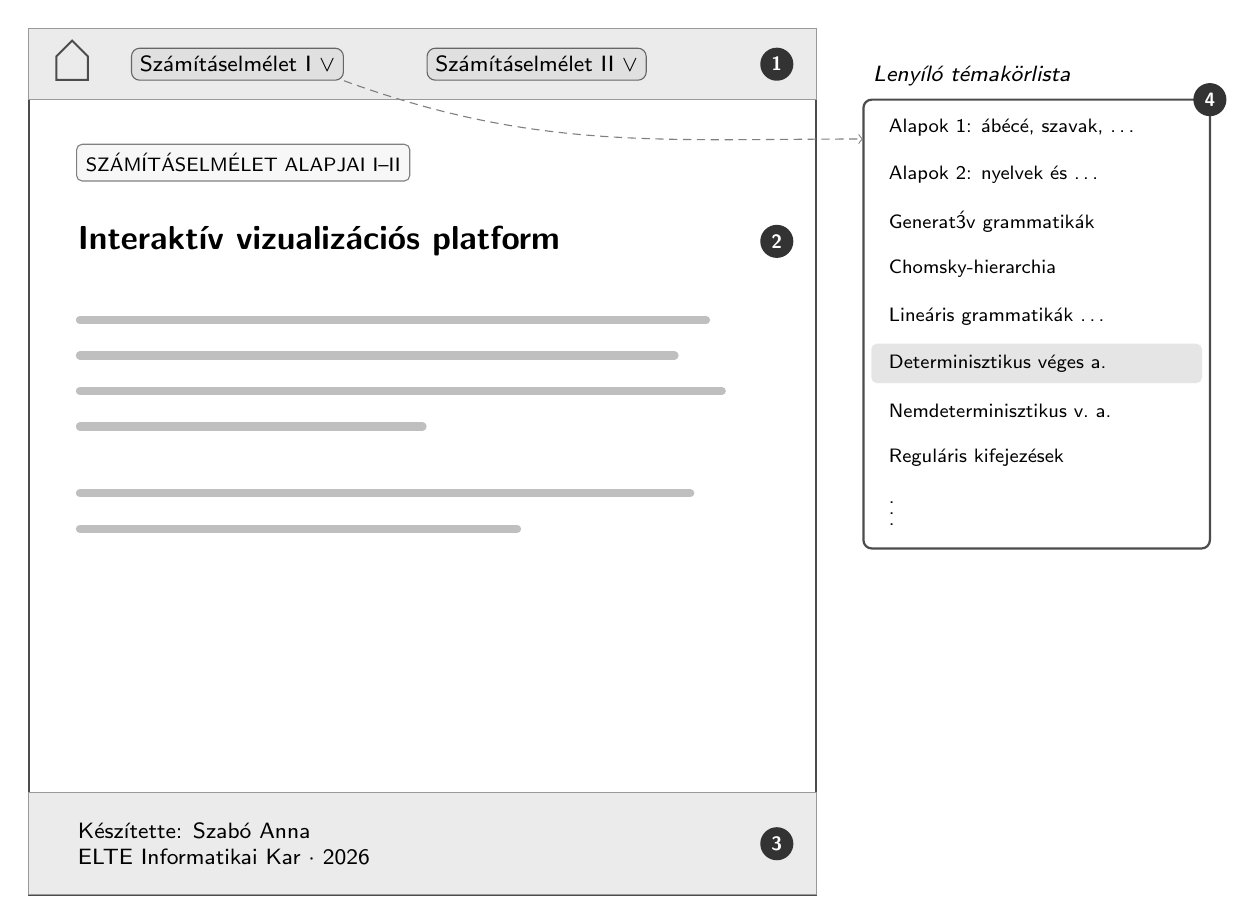
\begin{tikzpicture}[wf]
  \draw[wf frame] (0,0) rectangle (10,11);

  \draw[wf bar] (0,10.1) rectangle (10,11);
  \draw[black!70, line width=0.7pt] (0.35,10.35) -- (0.35,10.65) -- (0.55,10.85)
      -- (0.75,10.65) -- (0.75,10.35) -- cycle;
  \node[wf btn] (m1) at (2.65,10.55) {Számításelmélet I $\vee$};
  \node[wf btn] at (6.45,10.55) {Számításelmélet II $\vee$};
  \node[wf mark] at (9.5,10.55) {1};

  \node[wf box, anchor=west, font=\sffamily\scriptsize] at (0.6,9.3)
      {SZÁMÍTÁSELMÉLET ALAPJAI I--II};
  \node[anchor=west, font=\sffamily\large\bfseries] at (0.5,8.3)
      {Interaktív vizualizációs platform};
  \foreach \y/\l in {7.3/8.6, 6.85/8.2, 6.4/8.8, 5.95/5.0}
    \draw[wf line] (0.65,\y) -- (\l,\y);
  \foreach \y/\l in {5.1/8.4, 4.65/6.2}
    \draw[wf line] (0.65,\y) -- (\l,\y);
  \node[wf mark] at (9.5,8.3) {2};

  \draw[wf bar] (0,0) rectangle (10,1.3);
  \node[anchor=west, align=left] at (0.5,0.65)
      {Készítette: Szabó Anna\\ ELTE Informatikai Kar $\cdot$ 2026};
  \node[wf mark] at (9.5,0.65) {3};

  \begin{scope}[shift={(10.6,4.4)}]
    \node[anchor=south west, font=\sffamily\footnotesize\itshape] at (0,5.75)
        {Lenyíló témakörlista};
    \draw[wf frame, rounded corners=3pt] (0,0) rectangle (4.4,5.7);
    \fill[black!10, rounded corners=2pt] (0.1,2.1) rectangle (4.3,2.6);
    \foreach \t [count=\i] in {
        {Alapok 1: ábécé, szavak, \ldots},
        {Alapok 2: nyelvek és \ldots},
        Generatív grammatikák,
        Chomsky-hierarchia,
        Lineáris grammatikák \ldots,
        Determinisztikus véges a.,
        Nemdeterminisztikus v.\ a.,
        Reguláris kifejezések,
        \vdots}
      \node[anchor=west, font=\sffamily\scriptsize] at (0.2,5.95-0.6*\i) {\t};
    \node[wf mark] at (4.4,5.7) {4};
  \end{scope}
  \draw[densely dashed, black!50, ->] (m1.south east) to[out=-20, in=180] (10.6,9.6);
\end{tikzpicture}
}
    \caption{A főoldal vázlata}
    \label{fig:homepage}
\end{figure}

\clearpage

Egy témakör oldala (\ref{fig:module}.~ábra) felülről lefelé haladva
épül fel: (1) a helyet mutató morzsamenü és a cím, (2) az elméleti
összefoglaló tartalomblokkjai, (3) a \emph{Próbáld ki!} szakasz az
interaktív modullal, itt a bemeneti mezővel, a lejátszásvezérlővel és
az automata ábrájával, végül (4) a \emph{Teszteld magad!} szakasz a
kvízkérdésekkel. A (3) és (4) szakasz csak akkor jelenik meg, ha a
témakörhöz tartozik modul, illetve kvíz.

\begin{figure}[H]
    \centering
    \resizebox{!}{0.8\textheight}{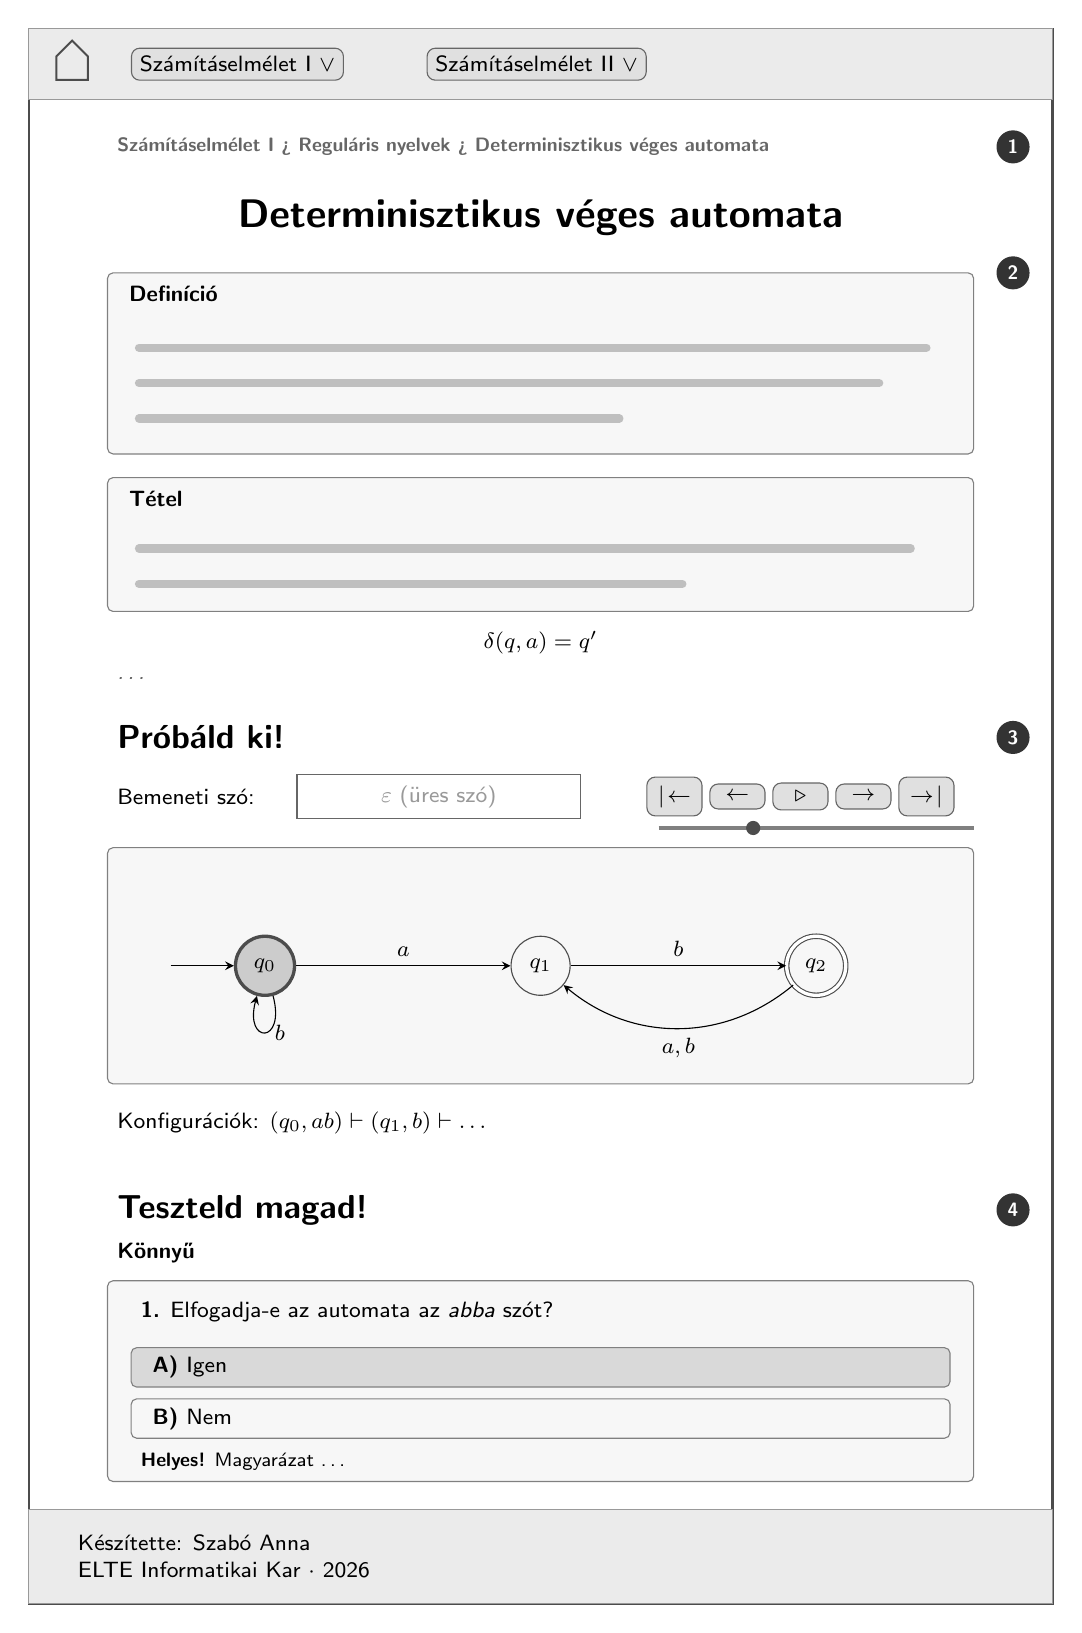
\begin{tikzpicture}[wf]
  \draw[wf frame] (0,0) rectangle (13,20);

  \draw[wf bar] (0,19.1) rectangle (13,20);
  \draw[black!70, line width=0.7pt] (0.35,19.35) -- (0.35,19.65) -- (0.55,19.85)
      -- (0.75,19.65) -- (0.75,19.35) -- cycle;
  \node[wf btn] at (2.65,19.55) {Számításelmélet I $\vee$};
  \node[wf btn] at (6.45,19.55) {Számításelmélet II $\vee$};

  \node[anchor=west, font=\sffamily\scriptsize\itshape\bfseries, black!60] at (1,18.5)
      {Számításelmélet I > Reguláris nyelvek > Determinisztikus véges automata};
  \node[wf mark] at (12.5,18.5) {1};
  \node[font=\sffamily\Large\bfseries] at (6.5,17.6) {Determinisztikus véges automata};

  \draw[wf box] (1,14.6) rectangle (12,16.9);
  \node[anchor=north west, font=\sffamily\footnotesize\bfseries] at (1.15,16.85) {Definíció};
  \foreach \y/\l in {15.95/11.4, 15.5/10.8, 15.05/7.5}
    \draw[wf line] (1.4,\y) -- (\l,\y);
  \draw[wf box] (1,12.6) rectangle (12,14.3);
  \node[anchor=north west, font=\sffamily\footnotesize\bfseries] at (1.15,14.25) {Tétel};
  \foreach \y/\l in {13.4/11.2, 12.95/8.3}
    \draw[wf line] (1.4,\y) -- (\l,\y);
  \node at (6.5,12.2) {$\delta(q, a) = q'$};
  \node[anchor=west, font=\sffamily\footnotesize\itshape, black!60] at (1,11.75) {\ldots};
  \node[wf mark] at (12.5,16.9) {2};

  \node[anchor=west, font=\sffamily\large\bfseries] at (1,11.0) {Próbáld ki!};
  \node[wf mark] at (12.5,11.0) {3};
  \node[anchor=west] at (1,10.25) {Bemeneti szó:};
  \node[wf input, minimum width=3.6cm] at (3.4,10.25) {\textcolor{black!40}{$\varepsilon$ (üres szó)}};
  \foreach \s [count=\i] in {{$|\!\leftarrow$}, {$\leftarrow$}, {$\triangleright$}, {$\rightarrow$}, {$\rightarrow\!|$}}
    \node[wf btn, minimum width=0.7cm] at (7.4+0.8*\i,10.25) {\s};
  \draw[black!50, line width=1.5pt] (8.0,9.85) -- (12,9.85);
  \fill[black!70] (9.2,9.85) circle (0.09);

  \draw[wf box] (1,6.6) rectangle (12,9.6);
  \node[wf state, fill=black!20, line width=1.2pt] (q0) at (3,8.1) {$q_0$};
  \node[wf state] (q1) at (6.5,8.1) {$q_1$};
  \node[wf state, double, double distance=1.2pt] (q2) at (10,8.1) {$q_2$};
  \draw[->, >=stealth] (1.8,8.1) -- (q0);
  \draw[->, >=stealth] (q0) -- node[above] {$a$} (q1);
  \draw[->, >=stealth] (q1) -- node[above] {$b$} (q2);
  \draw[->, >=stealth] (q0) to[loop below] node[right] {$b$} (q0);
  \draw[->, >=stealth] (q2) to[out=-140, in=-40] node[below] {$a, b$} (q1);
  \node[anchor=west] at (1,6.1) {Konfigurációk: $(q_0, ab) \vdash (q_1, b) \vdash \ldots$};

  \node[anchor=west, font=\sffamily\large\bfseries] at (1,5.0) {Teszteld magad!};
  \node[wf mark] at (12.5,5.0) {4};
  \node[anchor=west, font=\sffamily\footnotesize\bfseries] at (1,4.45) {Könnyű};
  \draw[wf box] (1,1.55) rectangle (12,4.1);
  \node[anchor=west] at (1.3,3.7) {\textbf{1.} Elfogadja-e az automata az \emph{abba} szót?};
  \draw[draw=black!50, fill=black!15, rounded corners=2pt] (1.3,2.75) rectangle (11.7,3.25);
  \node[anchor=west] at (1.45,3.0) {\textbf{A)} Igen};
  \draw[draw=black!50, rounded corners=2pt] (1.3,2.1) rectangle (11.7,2.6);
  \node[anchor=west] at (1.45,2.35) {\textbf{B)} Nem};
  \node[anchor=west, font=\sffamily\scriptsize] at (1.3,1.8) {\textbf{Helyes!} Magyarázat \ldots};

  \draw[wf bar] (0,0) rectangle (13,1.2);
  \node[anchor=west, align=left] at (0.5,0.6)
      {Készítette: Szabó Anna\\ ELTE Informatikai Kar $\cdot$ 2026};
\end{tikzpicture}
}
    \caption{Egy témakör oldalának vázlata}
    \label{fig:module}
\end{figure}

\subsubsection{Adatformátum: a tartalommodell}
\label{sec:data}

A tervezés fő szempontjai a következők voltak:

\begin{itemize}
    \item a tartalom legyen független a megjelenítéstől a UI-tól;
    \item a tananyag legyen könnyen bővíthető;
    \item a teljes tananyag egységes formátumban tárolódjon;
    \item az interaktív modulok (DVA, NDVA, veremautomata stb.)
          ráépíthetők legyenek.
\end{itemize}

A tananyag egymásba ágyazott egységekből álljon: a témakörök
csoportokba tartoznak, minden témakör elméleti anyaga tartalomblokkok
sorozatából épül fel, tartozhatnak hozzá kvízkérdések, illetve interaktív
modul. A felhasználó haladása ettől függetlenül, a böngészőben
tárolódik. Az egyes egységeket a~\ref{tab:data-logical}.~táblázat
mutatja be.

\begin{table}[H]
    \centering
    \begin{tabularx}{\textwidth}{|l|>{\raggedright\arraybackslash}X|>{\raggedright\arraybackslash}X|}
        \hline
        \textbf{Egység} & \textbf{Mit tartalmaz} & \textbf{Példa} \\
        \hline
        Témakörcsoport & a tárgy egy nagyobb része
                       & Reguláris nyelvek \\ \hline
        Témakör        & cím, rövid összefoglaló, kapcsolódó előadások,
                         kapcsolódó interaktív modul
                       & Determinisztikus véges automaták, a hozzá
                         tartozó DVA-szimulátorral \\ \hline
        Tartalomblokk  & magának az elméleti anyag egy eleme (definíció, tétel,
                         bizonyítás, példa, képlet, táblázat \ldots)
                       & a DVA definíciója \\ \hline
        Kvízkérdés     & kérdés, válaszlehetőségek, helyes válasz,
                         magyarázat
                       & „Elfogadja-e az automata az \emph{abba} szót?” \\ \hline
        Haladás        & a megoldott feladatok és a beállítások, megtekintett témakörök
                       & melyik kvíz lett már kitöltve \\
        \hline
    \end{tabularx}
    \caption{A tananyag felépítése}
    \label{tab:data-logical}
\end{table}


%----------------------------------------------------------------------
\subsection{A követelmények validációja}
%----------------------------------------------------------------------
% ea02, 40. dia: prototípus + tesztesetek
% - a fejlesztés iteratív prototípusokban haladt
% - a felhasználói történetekből lesznek a funkcionális tesztesetek -> Tesztelés fejezet
A fejezetben kifejtett követelmények validálásának célja annak ellenőrzése,
 hogy a megfogalmazott követelmények megvalósíthatók, egymással összhangban
  állnak-e, valamint lefedik a rendszer célkitűzéseit.
   A követelmények összevetésre kerültek a projekt céljaival és a 
   meghatározott hatókörökkel. 
   Ennek eredményeként minden célkitűzéshez kapcsolódik legalább 
   egy funkcionális követelmény, továbbá nem szerepel olyan követelmény, 
   amely ellentmondana a hatókörön kívül eső funkcióknak. 
   A követelmények teljesülésének ellenőrzése a fejlesztés során 
   egységtesztek, manuális tesztesetek és a rendszer gyakorlati 
   kipróbálása segítségével történik.
    A részletes tesztelési eredményeket a Tesztelés fejezet ismerteti később.
    %======================================================================
\section{Tervezés}
\iffalse
%======================================================================
% TODO: ide megy át a thesis.tex "Áttekintés" (3 csomag + modulregiszter)
% és a "Rendszerarchitektúra" fejezet

\subsection{A tartalommodell}
\label{sec:content-design}

A blokkalapú modell előnye, hogy minden témakör ugyanazzal a
megjelenítő komponenssel rajzolható ki, új tartalom felvétele egyszerű,
és egy későbbi export (például PDF vagy nyomtatható nézet) is könnyen
megoldható.

A tananyagot TypeScript-modulokban tárolom. A szerkezet JSON-kompatibilis
(csak objektumokat, tömböket, szövegeket és számokat használ), de a
TypeScript-típusok miatt a fordító már szerkesztés közben jelzi, ha
egy blokk hiányos vagy hibás.

\subsubsection{Többnyelvű szöveg}

Minden megjelenő szöveg \texttt{LocalizedText} típusú. A magyar
változat kötelező, az angol opcionális, így a fordítás a meglévő
tartalom módosítása nélkül, fokozatosan pótolható.

\begin{lstlisting}
type LocalizedText = {
  hu: string;
  en?: string;
};
\end{lstlisting}

\subsubsection{Tartalomblokkok}

Egy témakör elméleti anyaga \texttt{ContentBlock} elemek sorozata.
A \texttt{ContentBlock} ún.\ diszkriminált unió (\emph{discriminated
union}): minden blokknak van egy \texttt{type} mezője, amely alapján a
fordító és a megjelenítő is el tudja dönteni, milyen további mezői
vannak. A jelenleg definiált blokktípusokat
a~\ref{tab:blocks}.~táblázat mutatja.

\begin{table}[H]
    \centering
    \begin{tabularx}{\textwidth}{|l|p{4.6cm}|X|}
        \hline
        \textbf{\texttt{type}} & \textbf{Mezők} & \textbf{Szerep} \\
        \hline
        \texttt{heading}    & \texttt{level} (1--3), \texttt{text}
                            & Fejezet- vagy szakaszcím \\ \hline
        \texttt{paragraph}  & \texttt{text}
                            & Folyó szöveg \\ \hline
        \texttt{definition} & \texttt{term}, \texttt{content}
                            & Fogalom definíciója \\ \hline
        \texttt{theorem}    & \texttt{kind}, \texttt{name?},
                              \texttt{statement}, \texttt{proof?}
                            & Tétel, lemma, állítás vagy következmény \\ \hline
        \texttt{proof}      & \texttt{title?}, \texttt{content}
                            & Bizonyítás, maga is blokkok sorozata \\ \hline
        \texttt{example}    & \texttt{title?}, \texttt{content}
                            & Kidolgozott példa \\ \hline
        \texttt{formula}    & \texttt{latex}
                            & Kiemelt képlet \\ \hline
        \texttt{list}       & \texttt{ordered}, \texttt{items}
                            & Számozott vagy felsorolásos lista \\ \hline
        \texttt{table}      & \texttt{headers}, \texttt{rows}
                            & Táblázat (pl.\ átmenettáblázat) \\ \hline
        \texttt{warning}    & \texttt{text}
                            & Figyelmeztetés tipikus hibára \\ \hline
        \texttt{funfact}    & \texttt{text}
                            & Érdekesség, kiegészítő megjegyzés \\
        \hline
    \end{tabularx}
    \caption{A tartalomblokkok típusai (a \texttt{?} opcionális mezőt jelöl)}
    \label{tab:blocks}
\end{table}

A \texttt{theorem} blokk \texttt{kind} mezője a
\texttt{tetel}, \texttt{lemma}, \texttt{allitas} és
\texttt{kovetkezmeny} értékek egyikét veheti fel. Egy definíció például
így néz ki:

\begin{lstlisting}
{
  type: "definition",
  term: { hu: "Determinisztikus véges automata" },
  content: { hu: "Az $A = \\langle Q, \\Sigma, \\delta, q_0, F \\rangle$ rendezett ötös, ahol ..." },
}
\end{lstlisting}

\subsubsection{Matematikai jelölések}

A tárgy anyaga sok matematikai jelölést tartalmaz (automaták
definíciói, grammatikák, pumpálási lemmák, a CYK algoritmus stb.),
ezért a képleteket egységesen \LaTeX{} szintaxissal tárolom:

\begin{itemize}
    \item szövegen belüli képlet: \verb|$...$| a szövegmezőben;
    \item kiemelt képlet: külön \texttt{formula} blokk;
    \item a sztringekben a \verb|\| karaktert duplán kell írni
          (\verb|\\|).
\end{itemize}

\subsubsection{Témakörök metaadatai}

A tartalom és a navigáció szétválasztása érdekében minden témakörhöz
külön metaadat (\texttt{TopicMeta}) tartozik. Ez szolgál a
navigációhoz, a sorrendezéshez, a csoportosításhoz, az előadásokhoz
kötéshez, és ezen keresztül kapcsolódik a témakörhöz az
interaktív modul. Egy témakör (\texttt{Topic}) a metaadatokból, a
tartalomblokkok listájából és opcionálisan kvízkérdésekből áll.

\begin{table}[H]
    \centering
    \begin{tabularx}{\textwidth}{|l|l|X|}
        \hline
        \textbf{Mező} & \textbf{Típus} & \textbf{Jelentés} \\
        \hline
        \texttt{id}       & \texttt{string}        & Egyedi azonosító, az URL-ben is ez szerepel \\ \hline
        \texttt{order}    & \texttt{number}        & Megjelenési sorrend \\ \hline
        \texttt{group}    & \texttt{TopicGroup}    & Témakörcsoport \\ \hline
        \texttt{title}    & \texttt{LocalizedText} & Cím \\ \hline
        \texttt{summary}  & \texttt{LocalizedText} & Rövid összefoglaló \\ \hline
        \texttt{lectures} & \texttt{number[]}      & Kapcsolódó előadások sorszáma \\ \hline
        \texttt{module}   & \texttt{string | null} & A kapcsolódó interaktív modul azonosítója \\
        \hline
    \end{tabularx}
    \caption{A \texttt{TopicMeta} mezői}
    \label{tab:topicmeta}
\end{table}

A témakörök a tárgy logikai felosztását követve öt csoportba
(\texttt{TopicGroup}) sorolódnak:

\begin{table}[H]
    \centering
    \begin{tabular}{|l|l|}
        \hline
        \textbf{Azonosító} & \textbf{Jelentés} \\
        \hline
        \texttt{foundations}       & Alapfogalmak \\ \hline
        \texttt{regular}           & Reguláris nyelvek \\ \hline
        \texttt{context-free}      & Környezetfüggetlen nyelvek \\ \hline
        \texttt{context-sensitive} & Környezetfüggő és 0-típusú nyelvek \\ \hline
        \texttt{computability}     & Kiszámíthatóság (II. rész) \\
        \hline
    \end{tabular}
    \caption{Témakörcsoportok}
    \label{tab:groups}
\end{table}

% TODO: témakörök száma és listája a végén (most 16 mappa a topics/ alatt)  \fi
\cleardoublepage

\chapter{Összegzés}
\label{ch:sum}
\mbox{}

% Kb. 1 oldal: a probléma röviden, mit és hogyan csináltam, mire jutottam.

\chapter{Továbbfejlesztési lehetőségek}
\label{ch:future}
\mbox{}

% Kb. 1 oldal: Turing-gép modul, logika modul (igazságtáblák), veremautomata-szimulátor, további témakörök, grafikus automataszerkesztő.

\cleardoublepage

\nocite{*}
\phantomsection
\addcontentsline{toc}{chapter}{\biblabel}
\printbibliography[title=\biblabel]
\cleardoublepage

\phantomsection
\addcontentsline{toc}{chapter}{\lstfigurelabel}
\listoffigures
\cleardoublepage

\phantomsection
\addcontentsline{toc}{chapter}{\lsttablelabel}
\listoftables
\cleardoublepage

\end{document}
